
%\documentclass[11pts,a4paper,amsmath,amssymb,floatfix]{article}%{report}%{book}
\documentclass[12pts,a4paper,amsmath,amssymb,floatfix]{article}%{report}%{book}
\usepackage{graphicx,wrapfig,pdfpages}% Include figure files
%\usepackage{dcolumn,enumerate}% Align table columns on decimal point
%\usepackage{enumerate,enumitem}% Align table columns on decimal point
\usepackage{pdfpages,enumerate,enumitem}
\usepackage{bm,dpfloat}% bold math
\usepackage[pdftex,bookmarks,colorlinks=true,urlcolor=rltblue,citecolor=blue]{hyperref}
\usepackage{amsfonts,amsmath,amssymb,stmaryrd,indentfirst}
\usepackage{times,psfrag}
\usepackage{natbib}
\usepackage{color}
\usepackage{units}
\usepackage{rotating}
\usepackage{multirow}


\usepackage{pifont}
\usepackage{subfigure}
\usepackage{subeqnarray}
\usepackage{ifthen}

\usepackage{supertabular}
\usepackage{moreverb}
\usepackage{listings}
\usepackage{palatino}
%\usepackage{doi}
\usepackage{longtable}
\usepackage{float}
\usepackage{perpage}
\MakeSorted{figure}
%\usepackage{pdflscape}


%\usepackage{booktabs}
%\newcommand{\ra}[1]{\renewcommand{\arraystretch}{#1}}


\definecolor{rltblue}{rgb}{0,0,0.75}


%\usepackage{natbib}
\usepackage{fancyhdr} %%%%
\pagestyle{fancy}%%%%
% with this we ensure that the chapter and section
% headings are in lowercase
%%%%\renewcommand{\chaptermark}[1]{\markboth{#1}{}}
\renewcommand{\sectionmark}[1]{\markright{\thesection\ #1}}
\fancyhf{} %delete the current section for header and footer
\fancyhead[LE,RO]{\bfseries\thepage}
\fancyhead[LO]{\bfseries\rightmark}
\fancyhead[RE]{\bfseries\leftmark}
\renewcommand{\headrulewidth}{0.5pt}
% make space for the rule
\fancypagestyle{plain}{%
\fancyhead{} %get rid of the headers on plain pages
\renewcommand{\headrulewidth}{0pt} % and the line
}

\def\newblock{\hskip .11em plus .33em minus .07em}
\usepackage{color}

%\usepackage{makeidx}
%\makeindex

\setlength\textwidth      {16.cm}
\setlength\textheight     {22.6cm}
\setlength\oddsidemargin  {-0.3cm}
\setlength\evensidemargin {0.3cm}

\setlength\headheight{14.49998pt} 
\setlength\topmargin{0.0cm}
\setlength\headsep{1.cm}
\setlength\footskip{1.cm}
\setlength\parskip{0pt}
\setlength\parindent{0pt}


%%%
%%% Headers and Footers
\lhead[] {\text{\small{EG501J -- Geothermal Energy}}} 
\rhead[] {{\text{\small{Tutorial 03}}}}
%\chead[] {\text{\small{Session 2012/13}}} 
\lfoot[]{Dr Jeff Gomes}
%\cfoot[\thepage]{\thepage}
\rfoot[\text{\small{\thepage}}]{\thepage}
\renewcommand{\headrulewidth}{0.8pt}


%%%
%%% space between lines
%%%
\renewcommand{\baselinestretch}{1.5}

\newenvironment{VarDescription}[1]%
  {\begin{list}{}{\renewcommand{\makelabel}[1]{\textbf{##1:}\hfil}%
    \settowidth{\labelwidth}{\textbf{#1:}}%
    \setlength{\leftmargin}{\labelwidth}\addtolength{\leftmargin}{\labelsep}}}%
  {\end{list}}

%%%%%%%%%%%%%%%%%%%%%%%%%%%%%%%%%%%%%%%%%%%
%%%%%%                              %%%%%%%
%%%%%%      NOTATION SECTION        %%%%%%%
%%%%%%                              %%%%%%%
%%%%%%%%%%%%%%%%%%%%%%%%%%%%%%%%%%%%%%%%%%%

% Text abbreviations.
\newcommand{\ie}{{\em{i.e., }}}
\newcommand{\eg}{{\em{e.g., }}}
\newcommand{\cf}{{\em{cf., }}}
\newcommand{\wrt}{with respect to}
\newcommand{\lhs}{left hand side}
\newcommand{\rhs}{right hand side}
% Commands definining mathematical notation.

% This is for quantities which are physically vectors.
\renewcommand{\vec}[1]{{\mbox{\boldmath$#1$}}}
% Physical rank 2 tensors
\newcommand{\tensor}[1]{\overline{\overline{#1}}}
% This is for vectors formed of the value of a quantity at each node.
\newcommand{\dvec}[1]{\underline{#1}}
% This is for matrices in the discrete system.
\newcommand{\mat}[1]{\mathrm{#1}}


\DeclareMathOperator{\sgn}{sgn}
\newtheorem{thm}{Theorem}[section]
\newtheorem{lemma}[thm]{Lemma}

%\newcommand\qed{\hfill\mbox{$\Box$}}
\newcommand{\re}{{\mathrm{I}\hspace{-0.2em}\mathrm{R}}}
\newcommand{\inner}[2]{\langle#1,#2\rangle}
\renewcommand\leq{\leqslant}
\renewcommand\geq{\geqslant}
\renewcommand\le{\leqslant}
\renewcommand\ge{\geqslant}
\renewcommand\epsilon{\varepsilon}
\newcommand\eps{\varepsilon}
%\renewcommand\phi{\varphi}
\newcommand{\bmF}{\vec{F}}
\newcommand{\bmphi}{\vec{\phi}}
\newcommand{\bmn}{\vec{n}}
\newcommand{\bmns}{{\textrm{\scriptsize{\boldmath $n$}}}}
\newcommand{\bmi}{\vec{i}}
\newcommand{\bmj}{\vec{j}}
\newcommand{\bmk}{\vec{k}}
\newcommand{\bmx}{\vec{x}}
\newcommand{\bmu}{\vec{u}}
\newcommand{\bmv}{\vec{v}}
\newcommand{\bmr}{\vec{r}}
\newcommand{\bma}{\vec{a}}
\newcommand{\bmg}{\vec{g}}
\newcommand{\bmU}{\vec{U}}
\newcommand{\bmI}{\vec{I}}
\newcommand{\bmq}{\vec{q}}
\newcommand{\bmT}{\vec{T}}
\newcommand{\bmM}{\vec{M}}
\newcommand{\bmtau}{\vec{\tau}}
\newcommand{\bmOmega}{\vec{\Omega}}
\newcommand{\pp}{\partial}
\newcommand{\kaptens}{\tensor{\kappa}}
\newcommand{\tautens}{\tensor{\tau}}
\newcommand{\sigtens}{\tensor{\sigma}}
\newcommand{\etens}{\tensor{\dot\epsilon}}
\newcommand{\ktens}{\tensor{k}}
\newcommand{\half}{{\textstyle \frac{1}{2}}}
\newcommand{\tote}{E}
\newcommand{\inte}{e}
\newcommand{\strt}{\dot\epsilon}
\newcommand{\modu}{|\bmu|}
% Derivatives
\renewcommand{\d}{\mathrm{d}}
\newcommand{\D}{\mathrm{D}}
\newcommand{\ddx}[2][x]{\frac{\d#2}{\d#1}}
\newcommand{\ddxx}[2][x]{\frac{\d^2#2}{\d#1^2}}
\newcommand{\ddt}[2][t]{\frac{\d#2}{\d#1}}
\newcommand{\ddtt}[2][t]{\frac{\d^2#2}{\d#1^2}}
\newcommand{\ppx}[2][x]{\frac{\partial#2}{\partial#1}}
\newcommand{\ppxx}[2][x]{\frac{\partial^2#2}{\partial#1^2}}
\newcommand{\ppt}[2][t]{\frac{\partial#2}{\partial#1}}
\newcommand{\pptt}[2][t]{\frac{\partial^2#2}{\partial#1^2}}
\newcommand{\DDx}[2][x]{\frac{\D#2}{\D#1}}
\newcommand{\DDxx}[2][x]{\frac{\D^2#2}{\D#1^2}}
\newcommand{\DDt}[2][t]{\frac{\D#2}{\D#1}}
\newcommand{\DDtt}[2][t]{\frac{\D^2#2}{\D#1^2}}
% Norms
\newcommand{\Ltwo}{\ensuremath{L_2} }
% Basis functions
\newcommand{\Qone}{\ensuremath{Q_1} }
\newcommand{\Qtwo}{\ensuremath{Q_2} }
\newcommand{\Qthree}{\ensuremath{Q_3} }
\newcommand{\QN}{\ensuremath{Q_N} }
\newcommand{\Pzero}{\ensuremath{P_0} }
\newcommand{\Pone}{\ensuremath{P_1} }
\newcommand{\Ptwo}{\ensuremath{P_2} }
\newcommand{\Pthree}{\ensuremath{P_3} }
\newcommand{\PN}{\ensuremath{P_N} }
\newcommand{\Poo}{\ensuremath{P_1P_1} }
\newcommand{\PoDGPt}{\ensuremath{P_{-1}P_2} }

\newcommand{\metric}{\tensor{M}}
\newcommand{\configureflag}[1]{\texttt{#1}}

% Units
\newcommand{\m}[1][]{\unit[#1]{m}}
\newcommand{\km}[1][]{\unit[#1]{km}}
\newcommand{\s}[1][]{\unit[#1]{s}}
\newcommand{\invs}[1][]{\unit[#1]{s}\ensuremath{^{-1}}}
\newcommand{\ms}[1][]{\unit[#1]{m\ensuremath{\,}s\ensuremath{^{-1}}}}
\newcommand{\mss}[1][]{\unit[#1]{m\ensuremath{\,}s\ensuremath{^{-2}}}}
\newcommand{\K}[1][]{\unit[#1]{K}}
\newcommand{\PSU}[1][]{\unit[#1]{PSU}}
\newcommand{\Pa}[1][]{\unit[#1]{Pa}}
\newcommand{\kg}[1][]{\unit[#1]{kg}}
\newcommand{\rads}[1][]{\unit[#1]{rad\ensuremath{\,}s\ensuremath{^{-1}}}}
\newcommand{\kgmm}[1][]{\unit[#1]{kg\ensuremath{\,}m\ensuremath{^{-2}}}}
\newcommand{\kgmmm}[1][]{\unit[#1]{kg\ensuremath{\,}m\ensuremath{^{-3}}}}
\newcommand{\Nmm}[1][]{\unit[#1]{N\ensuremath{\,}m\ensuremath{^{-2}}}}

% Dimensionless numbers
\newcommand{\dimensionless}[1]{\mathrm{#1}}
\renewcommand{\Re}{\dimensionless{Re}}
\newcommand{\Ro}{\dimensionless{Ro}}
\newcommand{\Fr}{\dimensionless{Fr}}
\newcommand{\Bu}{\dimensionless{Bu}}
\newcommand{\Ri}{\dimensionless{Ri}}
\renewcommand{\Pr}{\dimensionless{Pr}}
\newcommand{\Pe}{\dimensionless{Pe}}
\newcommand{\Ek}{\dimensionless{Ek}}
\newcommand{\Gr}{\dimensionless{Gr}}
\newcommand{\Ra}{\dimensionless{Ra}}
\newcommand{\Sh}{\dimensionless{Sh}}
\newcommand{\Sc}{\dimensionless{Sc}}


% Journals
\newcommand{\IJHMT}{{\it International Journal of Heat and Mass Transfer}}
\newcommand{\NED}{{\it Nuclear Engineering and Design}}
\newcommand{\ICHMT}{{\it International Communications in Heat and Mass Transfer}}
\newcommand{\NET}{{\it Nuclear Engineering and Technology}}
\newcommand{\HT}{{\it Heat Transfer}}   
\newcommand{\IJHT}{{\it International Journal for Heat Transfer}}

\newcommand{\frc}{\displaystyle\frac}

\newlist{ExList}{enumerate}{1}
\setlist[ExList,1]{label={\bf Example 1.} {\bf \arabic*}}

\newlist{ProbList}{enumerate}{1}
\setlist[ProbList,1]{label={\bf Problem 1.} {\bf \arabic*}}

%%%%%%%%%%%%%%%%%%%%%%%%%%%%%%%%%%%%%%%%%%%
%%%%%%                              %%%%%%%
%%%%%% END OF THE NOTATION SECTION  %%%%%%%
%%%%%%                              %%%%%%%
%%%%%%%%%%%%%%%%%%%%%%%%%%%%%%%%%%%%%%%%%%%


% Cause numbering of subsubsections. 
%\setcounter{secnumdepth}{8}
%\setcounter{tocdepth}{8}

\setcounter{secnumdepth}{4}%
\setcounter{tocdepth}{4}%


\begin{document}



\begin{enumerate}[label=\bfseries Problem \arabic*:]

%%%
%%%
%%%
\item\label{PorousMedia} Figure~\ref{Fig:Binary} shows a schematic of a geothermal binary cycle operating with groundwater-steam (high temperature) and {\it isopentane} (low temperature) fluids in the dual cycle. 
\begin{enumerate}
\item $\lq$Cold groundwater' is injected in {\it injection well} whereas {\it hot water/steam} is recuperated in the {\it production well}. In other words, subcooled water displaces water/steam trapped in the porous media (or is heated up by hot geological formations), and this is driven to the production well. Discuss the set of physical phenomena in this process: 
\begin{itemize}
\item multiphase flow in porous media (Darcy law), 
\item phase change (thermodynamic dome, temperature $\times$ entropy and pressure $\times$ enthalpy diagrams) and,
\item heat transfer (conduction and convection) mechanisms.
\end{itemize}
\item Analyse the {\it isopentane} thermodynamic cycle. Assume it works in an ideal Rankine Cycle.
\end{enumerate}

\begin{figure}[h]
\begin{center}
  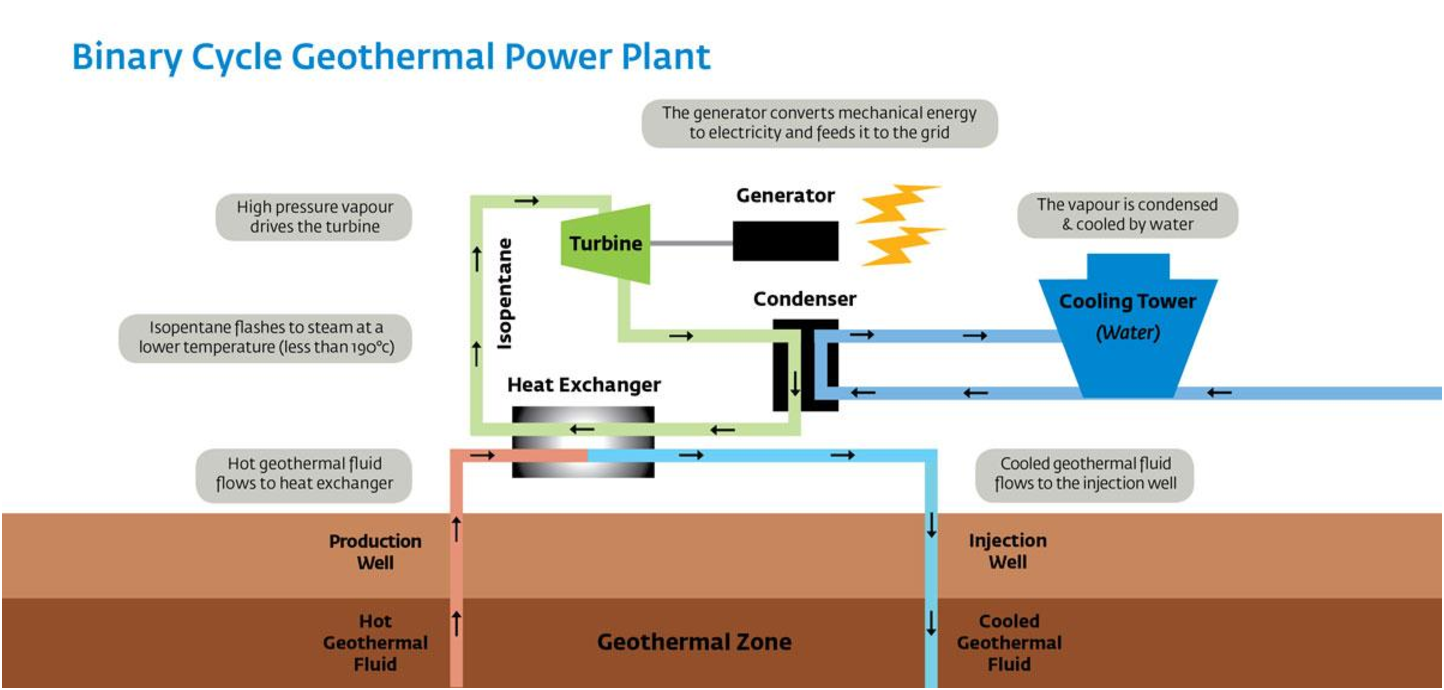
\includegraphics[width=12.0cm,height=7.0cm]{./Pics/BinaryCycle} 
\end{center}
\caption{Binary cycle: Problem~\ref{PorousMedia}.}\label{Fig:Binary}
\end{figure}

\clearpage

\noindent
    {\bf Solution:}
    \begin{enumerate}%[(a)]
%
    \item After heat is extracted from the geothermal fluid (\ie brine)\footnote{Brine is a generic name for groundwater with relatively high concentration of dissolved salts. These salts contain anions of: carbonates $\left(\text{CO}_{3}^{-2}\right)$, bicarbonates $\left(\text{HCO}_{3}^{-1}\right)$, chlorines  $\left(\text{Cl}^{-1}\right)$, chlorates  $\left(\text{ClO}_{3}^{-1}\right)$, sulfates $\left(\text{SO}_{4}^{-2}\right)$; and cations of: calcium $\left(\text{Ca}^{+2}\right)$, sodium  $\left(\text{Na}^{+1}\right)$, magnesium  $\left(\text{Mg}^{+2}\right)$, potassium  $\left(\text{K}^{+1}\right)$, etc. There are also silica $\left(\text{SiO}_{2}\right)$ and silicates, salts and oxides of arsenic and hydrigen sulfide $\left(\text{H}_{2}\text{S}\right)$.}, the excess of salts that were eventually concentrated during the process needs to be eliminated. This is due to environmental laws that constraint the maximum quantity of specific anions and cations that can be (re-)injected into the groundwater system. Environmental laws also determine the maximum temperature of the (re-)injected brine.

      Binary cycles are often operated with low-grade temperatures of 75-185$^{\circ}$C $\left(T_{H}\right)$ and use organic Rankine fluids (ORF) as working fluids. Brine temperature after heat transfer into the Rankine cycle is in the range of 70-120$^{\circ}$C (depending on the design of the heat exchanger). `Cold' brine (see previous paragraph on environmental laws restrictions) is injected into the well at a prescribed (relatively) high-pressure $\left(P_{0}\right)$, mass flow rate, $\left(\dot{m}_{w}\right)$ and depth $\left(z_{0}\right)$. At these conditions, brine is a saturated liquid and denser than brine at higher temperature, and as such it tends to move downwards, displacing hot and lighter brine upwards (thermal buoyancy). As `cold' brine is injected, it displaces `hot' and lighter brine towards the production well (due to pressure gradient), Fig.~\ref{SolutionProb1}(top).

      The non-inertia dominated flow of these fluids (hot and cold liquid brine in thermodynamic equilibrium with the vapour phases) in porous media is a multiphase flow system that can be described by the extended Darcy equation,
      \begin{equation}
        \underline{u}_{\alpha} = -\frc{\mathcal{K}\mathcal{K}_{r\alpha}}{\mu_{\alpha}}\left(\nabla \underline{p}_{\alpha} - \rho_{\alpha}\underline{g} + \mathcal{S}_{\text{mom},\alpha}\right),
      \end{equation}
      where $\underline{u}_{\alpha}$ is the Darcy velocity associated with phase $\alpha$, $\mathcal{K}$ is the absolute permeability, $\mu$ is the fluid viscosity, $\underline{p}$ is the pressure, $\rho$ is the fluid density, $\underline{g}$ is the gravity acceleration, $\mathcal{S}_{\text{mom}}$ are source and/or sink terms for the momentum equations, and $\mathcal{K}_{r\alpha}$ is the relative permeability (a functional that depends on the fluid saturation, $S_{\alpha}$, and rock properties). The extended Darcy Equation is coupled with the continuity equation (also called saturation equation),
      \begin{equation}
        \frc{\partial}{\partial t}\left(\phi\rho_{\alpha}S_{\alpha}\right) + \nabla\cdot\left(u_{\alpha}\rho_{\alpha}S_{\alpha}\right) = \mathcal{S}_{\text{cont},\alpha},
      \end{equation}
      where $\phi$ is the rock porosity and $\mathcal{S}_{\text{cont},\alpha}$ are source and/or source terms for the continuity equation. As brine is driven towards the production well, `cold' fluid extracts heat energy from deep rock formations (geothermal source), vaporising part of the liquid fraction and decreasing the density. The density of the brine at the well head at $T$ and $P$ is
      \begin{equation}
          \rho\left(T,P\right) = \rho_{L}S_{L}\left(T,P\right) +  \rho_{V}S_{V}\left(T,P\right),
      \end{equation} 
      where subscripts $L$ and $V$ stand for liquid and vapour phases. Figure~\ref{SolutionProb1} shows sketches of temperature $\times$ specific entropy ($Ts$) and pressure $\times$ enthalpy ($Ph$) diagrams of the subsurface flow (validity of these diagrams depend on conditions of geothermal fluid production). 
      \begin{figure}[h]
        \vbox{
          \hbox{\includegraphics[width=\columnwidth,clip]{./Pics/Tut3_Sketch}}
           \vspace{0.cm}
           \hbox{\includegraphics[width=.5\columnwidth,clip]{./Pics/Tut3_Sketch2}
                 \includegraphics[width=.5\columnwidth,clip]{./Pics/Tut3_Sketch3}}}
        \caption{~\ref{PorousMedia} sketch of subsurface flow (top) and associated $Ph$ and $Ts$ diagrams.}\label{SolutionProb1}
      \end{figure}
      
      From Fig.~\ref{SolutionProb2}, there are three main heat exchange mechanisms in geo-fluids,
      \begin{enumerate}
         \item thermal conduction;
         \item convection (or interphase heat transfer), and;
         \item thermal radiation (not explicitly shown in the figure) from Earth's core to rock formations at (relatively) large depths.
      \end{enumerate}
      Conduction mechanisms occur within the same phase (\eg solid-solid, liquid-liquid phases) and depend on surface contact between materials (\ie rocks of distinct geological nature) and are proportional to the temperature gradient,
      \begin{equation}
          Q_{\text{cond}} = - \kappa\nabla T,
      \end{equation}
      where $Q_{\text{cond}}$ is the heat transferred due to conduction and $\kappa$ is the thermal conductivity coefficient.  Thus heat from geothermal rock formations at great depth is transported through surface contact between rocks (see Fig.~\ref{SolutionProb3}). Heat transferred to lower depths (represented by layer $L_{3}$) lead to rock temperature $T_{3}$ at the interface with the rock saturated with fluids. As the temperature of such saturated geological formation $\left(T_{\text{rs}}\right)$ is smaller than $T_{3}$, heat is transferred from the interfacial layer to the saturated rock. Conductive heat transfer is also responsible for heat losses in the upper level of the geothermal reservoir (Fig.~\ref{SolutionProb2}, as conductive heat loss). 
      
      \begin{figure}[h]%
        \begin{center}
          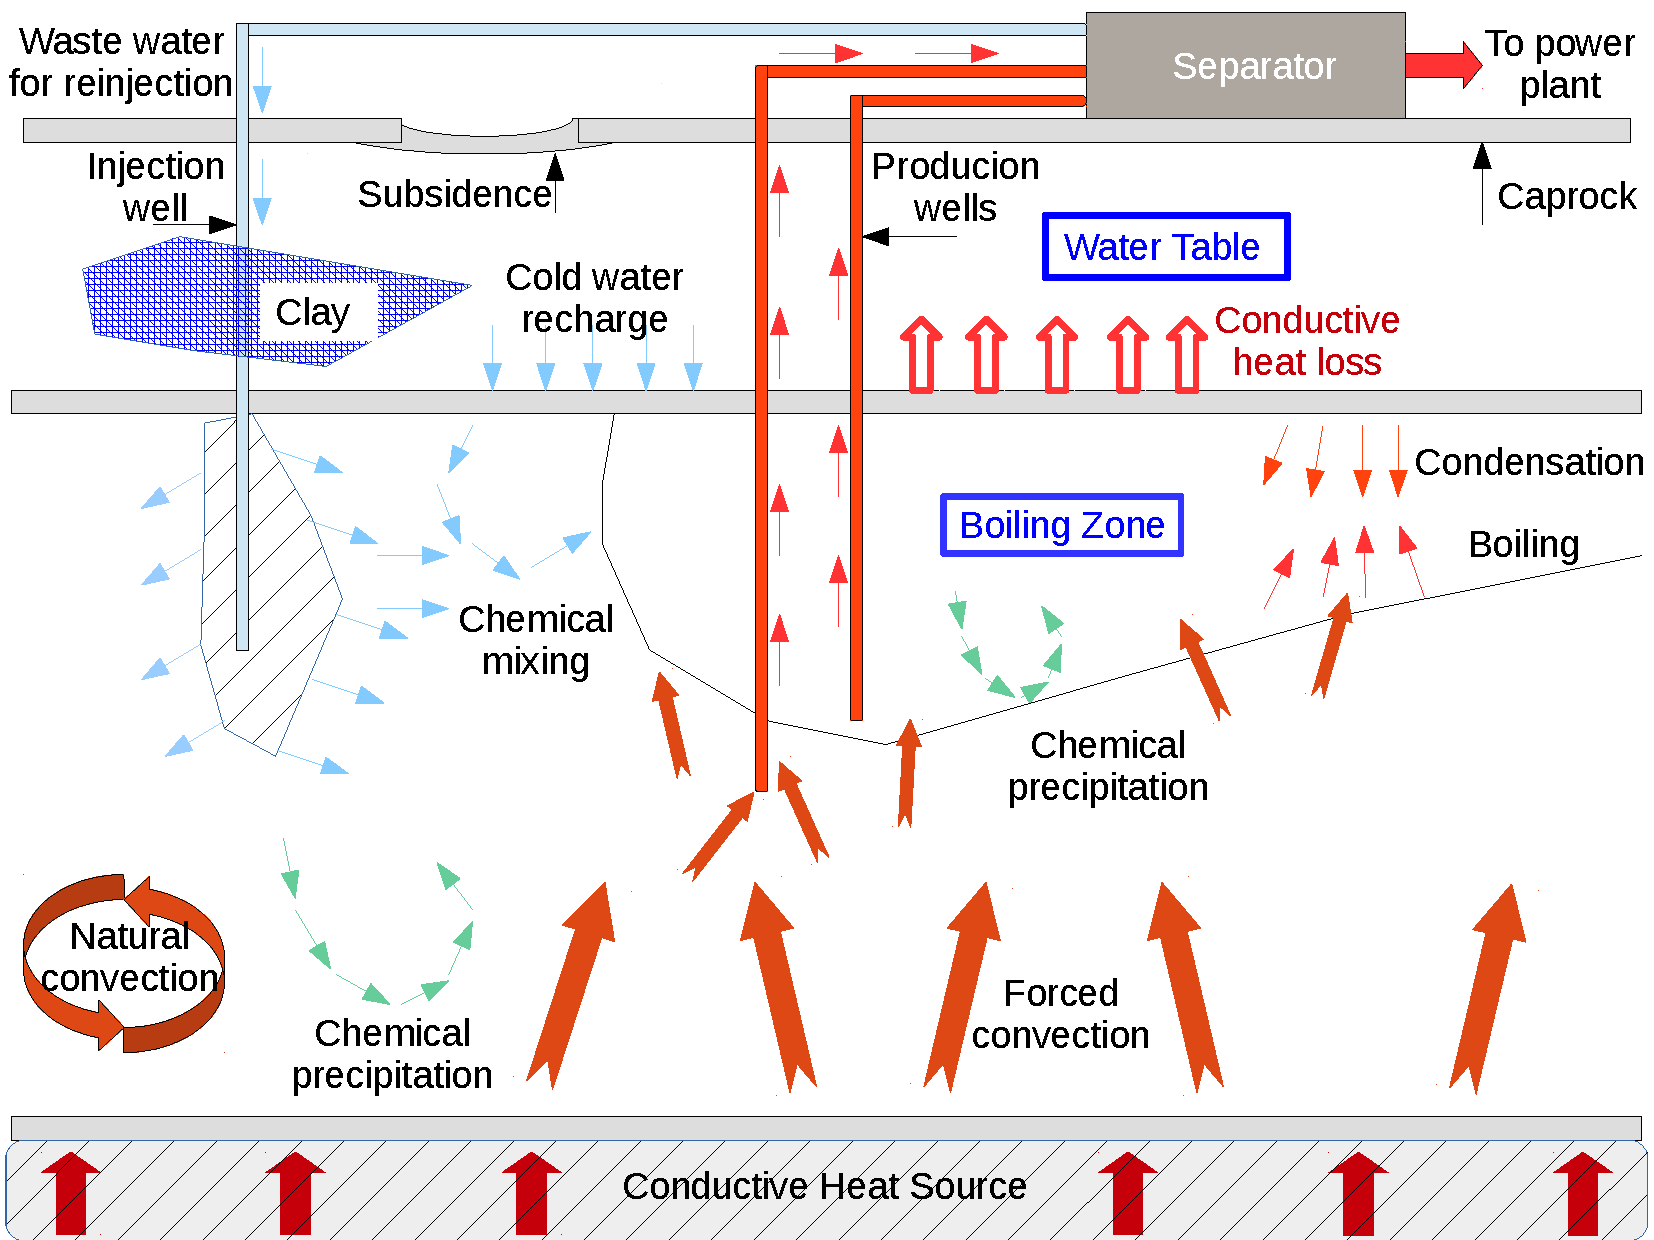
\includegraphics[width=\columnwidth, clip]{./Pics/GeothermalOverviewDiagram}
        \end{center}
        \caption{Schematics of physical phenomena in geothermal reservoirs.}\label{SolutionProb2}
      \end{figure}

      The difference in temperature between the interface rock $\left(T_{3}\right)$ and the temperature of rock saturated with fluids, $T_{\text{rs}}$ leads to the forced convective heat transfer. Here, assuming that rocks and fluids close to the interface are in thermal equilibrium,
      \begin{displaymath}
        T_{\text{rs}} = T_{\text{rock}} = T_{\text{fluid}},
      \end{displaymath}
      the convective (or interphase) heat transfer can be defined as
      \begin{equation}
         Q_{\text{conv}} = \mathcal{H}\Delta T =  \mathcal{H}\left(T_{3}-T_{\text{rs}}\right),
      \end{equation}
      where $\mathcal{H}$ is the convective heat transfer coefficient. As the fluid is heated up (and partially / totally vaporised), it becomes less dense and is moved upward by sinking `cold' denser fluid. This thermally induced circulation of fluids is called natural convection and is due to thermal buoyancy.      
      
      \begin{figure}[h]%
        \begin{center}
          \includegraphics[width=\columnwidth, clip]{./Pics/Tut3_Sketch4}
        \end{center}
        \caption{Schematics of conduction heat transfer from Earth's core to geothermal reservoir.}\label{SolutionProb3}
      \end{figure}

%
    \item In the power binary cycle with isopentane $\left(\text{i-C}_{5}\right)$ as working fluid (Fig.~\ref{SolutionProb4}), heat is extracted from the geothermal fluid in a heat exchanger $\left(\dot{Q}_{\text{hot}}\right)$. As all organic Rankine fluids, i-C$_{5}$ has a low boiling point ($\sim$ 28$^{\circ}$C) and is entirely vaporised. Depending on the geothermal fluid temperature and efficiency of the heat exchanger, i-C$_{5}$ can become superheated vapour with high associated enthalpy. This thermal energy (heat) is transformed into mechanical energy $\left(\dot{W}_{T}\right)$ in a (set of) turbine(s) as i-C$_{5}$ undertakes an isentropic expansion (\ie at constant entropy). The residual energy in the i-C$_{5}$ stream is extracted in a (set of) condenser(s) $\left(\dot{Q}_{\text{cond}}\right)$ and transferred to another fluid (\eg water) that is either released to the environment or transferred to other facilities. As the energy is extracted, the fluid that is partially condensed in $2$, becomes saturated liquid in $3$ (\ie after the condenser), allowing i-C$_{5}$ to be pumped back to the heat exchanger. The $Ts$ diagram is shown in Fig.~\ref{SolutionProb4} (bottom)
      \begin{figure}[h]
        \vbox{
          \hbox{\includegraphics[width=.8\columnwidth,clip]{./Pics/Tut3_Sketch5}}
           \vspace{0.cm}
           \hbox{\includegraphics[width=.8\columnwidth,clip]{./Pics/Tut3_Sketch6}}}
        \caption{Sketch of the power system and associated $Ts$ thermodynamic cycle (bottom).}\label{SolutionProb4}
      \end{figure}
      
%      
    \end{enumerate}
    


\clearpage 
%%%
%%%
%%%
\item\label{PorousMedia_Carman-Kozeny} After a heavy thunderstorm, water accumulated in a area located in the top of a water table.  The accumulated water slowly percolates the sandstone formation (15 m thick) of porosity 0.45 and mean particle diameter $\left(d_{s}\right)$ of 0.25 mm. Calculate the volumetric flow rate $\left(\text{m}^{3}.\text{s}^{-1}\right)$ using the Carman-Koneny equation,
\begin{displaymath}
    \frc{dp}{dz} = -180u \frc{\mu\left(1-\phi\right)^{2}}{d_{s}^{2}\phi^{3}},
\end{displaymath}
of an area of (1$\times$1) m$^{2}$, where $u$ is the fluid velocity. Dynamic viscosity, $\left(\mu\right)$ and density $\left(\rho\right)$ of water are 0.89 cP and 998 kg.m$^{-3}$, respectively. $z$ is the vertical depth, also the hydrostatic pressure in a fluid can be determined by,
\begin{displaymath}
  p = p_{0} +\rho g z
\end{displaymath}

{\bf Solution:} In this problem we need to calculate the volumetric flow rate of the rainwater through rock layers of sandstone formation, \ie
\begin{displaymath}
  \dot{Q} = \left|u\right| \times \text{Area},
\end{displaymath}
where $u$ is the fluid velocity. The first step to solve this problem is to ensure that all relevant variables have SI units,
\begin{displaymath}
   \mu = 0.89 \text{ cP} = 0.89\times 10^{-3} \frc{\text{N.s}}{\text{m}^{2}}\;\;\;\text{ and }\;\;\; d_{s} = 0.25\text{ mm} = 0.25\times 10^{-3}\text{ m}
\end{displaymath}
The Carman-Koneny equation gives a relationship between pressure drop through the porous media and velocity, 
\begin{displaymath}
    \frc{dp}{dz} = -180u \frc{\mu\left(1-\phi\right)^{2}}{d_{s}^{2}\phi^{3}},
\end{displaymath}
however, pressure drop $\frac{dp}{dz}$ is not known but can be obtained by manipulating the hydrostatic pressure equation,
\begin{displaymath}
    \frc{dP}{dz} = \rho g, 
\end{displaymath}
the equation above indicates that the reference origin is in the surface, therefore
\begin{eqnarray}
  \frc{dP}{dz} = \rho g &=& -180u \frc{\mu\left(1-\phi\right)^{2}}{d_{s}^{2}\phi^{3}} \nonumber \\
  998 \frc{\text{kg}}{\text{m}^{3}} \times 9.81\frc{\text{m}}{\text{s}^{2}} &=& - 180 \times u \times 0.89\times 10^{-3} \frc{\text{N.s}}{\text{m}^{2}} \frc{\left(1-0.45\right)^{2}}{\left(0.25\times 10^{\-3}\text{m}\right)^{2}\times 0.45^{3}} \times \frc{\frc{1\text{ kg.m}}{\text{s}^{2}}}{1\text{ N}} \nonumber \\
   u &=& -1.1506\times 10^{-3} \frc{\text{m}}{\text{s}}  \nonumber
\end{eqnarray}
The negative velocity indicates that the fluid flows downwards. Finally the volumetric flow rate is $\left(\text{with area of 1 m}^{2}\right)$
\begin{displaymath}
  \dot{Q} = \left|u\right| \times \text{Area} = 1.1506\times 10^{-3} \frc{\text{m}^{3}}{\text{s}}
\end{displaymath}



      \begin{figure}[h]%
        \begin{center}
          \includegraphics[width=\columnwidth, clip]{./Pics/Tut3_Sketch7}
        \end{center}
        \caption{Schematics of rainwater flow through sandstone.}\label{SolutionProb5}
      \end{figure}



\end{enumerate} 


\clearpage

%{
%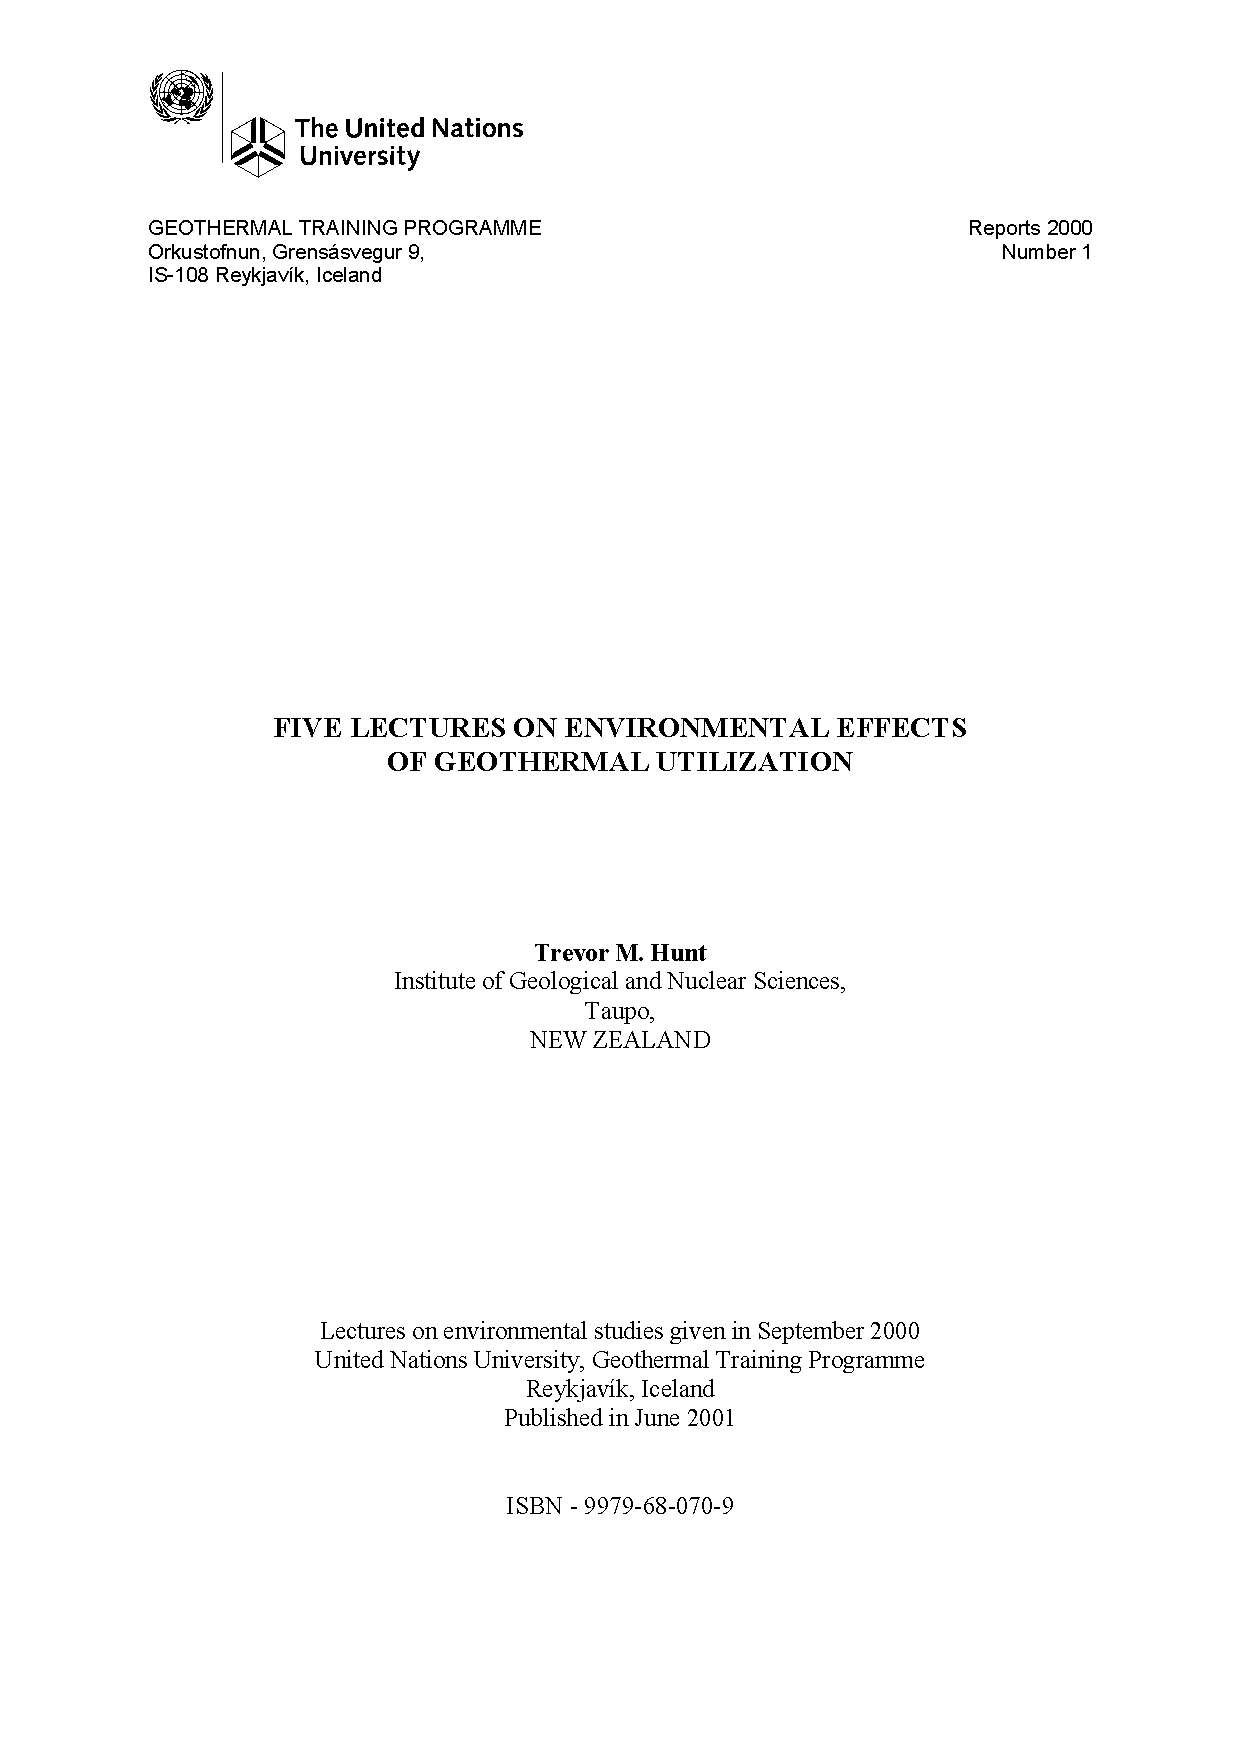
\includepdf[pages=-,fitpaper, angle=0]{./HuntSelect.pdf}
%}

\end{document}
